% Speaker script for slides.tex.  Build: ./build.sh
% build_html.py converts this file into notes.html and into the notes panel of
% slides.html, so keep to the macros used here (\slidenote, \emph, \textbf,
% inline $...$ with the symbols listed in build_html.MATH, ^{} and _{}).
% Everything from the first slide note up to the first new-page command is
% parsed; the backup part is separated with a clear-page command so that it
% stays in that range.
\documentclass[12pt,a4paper]{article}
\usepackage[T1]{fontenc}
\usepackage[utf8]{inputenc}
\usepackage{lmodern}
\usepackage[a4paper,margin=2.0cm]{geometry}
\usepackage{graphicx}
\usepackage{xcolor}
\usepackage{amsmath}
\usepackage{enumitem}
\usepackage[colorlinks=true,urlcolor=blue!55!black]{hyperref}
\definecolor{accent}{HTML}{1F5FA8}
\definecolor{muted}{HTML}{6B7280}
\setlength{\parindent}{0pt}
\setlength{\parskip}{6pt}
\linespread{1.12}

% \slidenote{page in slides.pdf}{label shown}{title}{timing}
\newcommand{\slidenote}[4]{%
  \par\bigskip\noindent
  \begin{minipage}[t]{.3\textwidth}\vspace{0pt}
    \includegraphics[page=#1,width=\linewidth]{slides.pdf}
  \end{minipage}\hfill
  \begin{minipage}[t]{.66\textwidth}\vspace{0pt}
    {\large\bfseries\color{accent}#2.\ #3}\par
    {\small\color{muted}#4}
  \end{minipage}\par\smallskip}


% Short lead sentence used at the top of each backup note.
\newcommand{\inone}[1]{\textbf{In one line.} #1\par}
\begin{document}

{\LARGE\bfseries Speaker script\par}
\smallskip
{\large Extremality shift of rotating black holes at finite Gauss--Bonnet coupling\par}
{\color{muted}Five minutes: five slides plus a closing one, about 700 words at a brisk but calm pace. The times are targets; the elapsed time is in brackets. The ``Background'' paragraph is for you and is not spoken. Slides A1--A5 are backup for questions. Their notes are short and plain; Appendices A and B at the end tell the same story in more detail.\par}

\slidenote{1}{1}{Title}{0:15 \quad [0:15]}

This is joint work with Cecilia Bejarano, David Blanco, Guillem Pérez-Nadal and
myself. Most of the code, the calculations and the writing were done by two AI
agents, Claude Code and Codex. We chose the question and checked the answers.

\slidenote{2}{2}{The question}{1:05 \quad [1:20]}

Start with a simple fact. A black hole cannot spin as fast as it likes for its
mass. There is a speed limit. A black hole sitting exactly at the limit is called
\emph{extremal}, and its temperature is zero.

In five dimensions, with two equal spins $J$, the limit says the mass must be at
least three halves of $\pi^{1/3} J^{2/3}$. That is the orange star.

This limit comes from Einstein's equations. Now add the simplest higher-curvature
correction, the Gauss--Bonnet term, with a strength $\alpha$. The limit moves. For
small $\alpha$ we already knew by how much: the smallest allowed mass grows with
slope exactly $\pi$. That is the dashed line.

But $\alpha$ does not have to be small. What happens then? That is the question
mark. A hint came from earlier numerical rotating black holes, which exist at
finite $\alpha$.

\textbf{Background: where the Gauss--Bonnet term comes from} (not spoken; use a
sentence of it if someone asks). Einstein's theory comes from the simplest
possible action: the curvature $R$ added up over spacetime. Its equations are
second order, like Newton's or Maxwell's. The Gauss--Bonnet term,
$L_{\rm GB} = R^2 - 4R_{\mu\nu}R^{\mu\nu} + R_{\mu\nu\rho\sigma}R^{\mu\nu\rho\sigma}$,
is the next simplest thing you can write: it is quadratic in the curvature. Such
terms are expected as the first corrections to general relativity in effective
field theory, and they appear in the low-energy limit of string theory. Their
strength $\alpha$ has units of length squared. Gauss--Bonnet is special because
its equations stay second order, and in four dimensions it changes nothing at
all. That is one reason to work in five dimensions.

\slidenote{3}{3}{Main result}{1:20 \quad [2:40]}

Here is our idea. Think of $\alpha$ as one more knob in thermodynamics, like
pressure or volume. Then the first law of black holes gets one more term,
$\Psi\,d\alpha$. The number $\Psi$ tells us how much the mass changes when we
turn the knob, keeping entropy and spin fixed.

At zero temperature the temperature term drops out. So, at fixed spin, $\Psi$ is
exactly the slope we want: how fast the smallest allowed mass grows with
$\alpha$.

We measured $\Psi$ on 356 numerical black holes, at 13 values of $\alpha$. We made
them colder and colder, and extrapolated to zero temperature.

The plot on the left is the answer. At $\alpha = 0$ we get back $\pi$, the green
star. Then the slope drops quickly, to about 1.07, and climbs again to 1.44 at
the largest coupling we reached.

Three messages. First, the slope is always positive, so Gauss--Bonnet tightens
the spin limit. Second, the slope is far from constant, so the first-order formula
fails quickly. Third, the slope is not monotonic: it falls and then rises. On the
right you see the smallest allowed mass itself. It grows by 31 percent. The
first-order line would predict more than twice that growth.

\slidenote{4}{4}{Validation}{1:10 \quad [3:50]}

How do we know this is right? Three kinds of evidence.

First, answers we already know. Our code reproduced a published family of
rotating black holes, to two parts in ten thousand at the horizon. It also gives
the exact static solution, and it gives $\pi$ when $\alpha$ is small.

Second, independent routes. We can get $\Psi$ in two other ways that do not use
our main method: from a scaling identity called the Smarr relation, and from an
integral of the Gauss--Bonnet curvature outside the black hole. Both agree with
our $\Psi$ to about one part in a million. The bars on the slide show the worst
disagreement of each check.

Third, the caveat. We never build a black hole at exactly zero temperature. We go
very cold and extrapolate. This is our biggest uncertainty. The bars on the result
plot show how much the answer moves when we extrapolate in different reasonable
ways.

\slidenote{5}{5}{What we learned with agents}{1:05 \quad [4:55]}

Finally, what we learned from working with agents. We chose the question and kept
doubting. Claude Code wrote and ran the code. Codex was the referee: it read the
results and asked for checks.

That mattered. One check the referee asked for actually failed. We had computed
the slope in two ways, and the two answers disagreed by more than our error bars.
So the bars were too small. We made them bigger, to cover every reasonable way of
doing the extrapolation.

Where did the effort go? Not where you might expect. Reproducing all the known
solutions took about 100 million tokens. The first new object, the rotating
solver, took five times more. In total, about 37 hours of agent time.

Our lesson: the cost is not writing code, it is checking it. Ask for checks that
can fail, and let one agent referee the other. Everything is in the repository.

\slidenote{6}{6}{Thank you}{0:05 \quad [5:00]}

Thank you for your attention, and thanks to Matías and Nahuel for the AI course.

\clearpage
{\Large\bfseries Backup slides}\par
{\color{muted}Not part of the five minutes. Each note is short and meant to be read, not recited. The long version is in Appendices A and B.\par}

\slidenote{7}{A1}{Numerical method: solving the field equations}{backup}

\inone{We turn a hard problem that depends on several directions into a short list of
ordinary equations along one direction, the radius, and let the computer solve
them.}

With two equal spins the black hole looks the same from many angles, so only the
radius matters. Four unknown functions describe it: $b$ (how fast time runs), $f$
(how radial distances stretch), $h$ (the size of the rotating circles) and $w$
(how fast space is dragged around). The equations stay second order, which is the
special property of Gauss--Bonnet.

At the horizon $b$ and $f$ vanish and $w$ equals the horizon's angular velocity
$\Omega_H$. Far away the space must be flat. We fix the horizon radius to 1; every
other size follows by rescaling.

The computer stores each function at 64 well-chosen points, crowded near the ends,
and demands that the equations hold there. That gives a few hundred ordinary
equations for as many numbers. We solve them with Newton's method (guess, measure
the error, correct) and we start from the exact Einstein solution and change
$\alpha$ gradually. A separate program then checks the original equations at 51
points \emph{between} the grid points; we keep a solution only if the error is
below $10^{-8}$. Mass and spin are read from how the fields fade away far from the
hole.

\emph{Left plot.} Before anything new, we had to reproduce a published family
(Brihaye, Kleihaus, Kunz and Radu, 2010). Lines are ours, circles are theirs. They
agree to $2\times10^{-4}$ at the horizon. In the interior they differ by up to
$1.4\times10^{-2}$, and we do not know why: their own curve near zero coupling is
already $9.5\times10^{-3}$ away from the exact formula, so their plot cannot test
ours more sharply than about one percent. One number in their text, an ergosurface
radius, does not match ours (1.1021 against 1.104). We report it as open. It does
not enter $\Psi$.

\emph{Right plot.} The same four functions at all 13 couplings. The change is not
small: at the largest coupling the horizon is squashed the opposite way from the
Einstein one.

\slidenote{8}{A2}{Numerical method: measuring $\Psi$ and reaching $T = 0$}{backup}

\inone{$\Psi$ comes from one extra linear solve, with no step size, and $T = 0$
comes from extrapolating.}

$\Psi$ is the change in mass when we change the theory, at fixed entropy and spin.
But the code holds the horizon radius and angular velocity fixed instead, and then
entropy and spin change too. The first law tells us how to subtract those
changes; what is left is $\Psi$. The factor 2 counts the two equal spins.

The static black hole shows why this matters. At fixed radius its mass grows with
$\alpha$, yet $\Psi$ is negative ($-9\pi/4$ for small $\alpha$). Holding the radius
fixed and holding the entropy fixed are different comparisons.

To get the derivatives we do not solve twice and subtract. That needs a step size,
and it is fragile near zero temperature. Instead we use a simple fact: the
equations hold for every $\alpha$, so if we nudge $\alpha$ the solution must move
just enough to keep them true. One linear solve, using the matrix that Newton's
method already built, tells us how much. We checked it against ordinary
differences: the gap shrinks by about four each time the step is halved, as it
should.

For the last step we cannot run the code at $T = 0$, where the horizon is
degenerate. We go as cold as possible, about $3\times10^{-6}$ in scaled units, fit
a smooth curve through the six coldest points, and read the value at zero. The
bars come from repeating the fit in 20 other reasonable ways.

\slidenote{9}{A3}{Physical meaning of the result}{backup}

\inone{A positive slope means Gauss--Bonnet black holes can spin less than Einstein
ones; the dip marks the fastest-rotating extremal horizon; the later rise is
consistent with a mass floor.}

\textbf{The sign.} A positive slope means the smallest allowed mass grows with
$\alpha$. The same statement read the other way: for a given mass, the largest
allowed spin goes down. On the right plot, the red curve starts at 1 (the Einstein
limit) and falls.

\textbf{Smarr relation.} At zero temperature a scaling identity reads
$\alpha\Psi_{\rm ext} = M_{\rm ext} - 3\Omega_H J$. In Einstein gravity the right
side is zero. A positive slope means Gauss--Bonnet opens a gap between the mass and
the rotational term, and the gap keeps growing, first quickly and then more slowly.

\textbf{The dip.} Rewriting that identity in scale-free variables gives
$3\omega = \mu - y\mu'$, where $\omega$ is the horizon's angular velocity in
natural units. Differentiating shows that the lowest slope is exactly the
highest $\omega$: the extremal black hole whose horizon spins fastest. The
data agree.

\textbf{The rise.} Static Gauss--Bonnet black holes cannot be lighter than
$3\pi\alpha/4$, and Kleihaus, Kunz and Radu report the same for rotating ones. Since the smallest mass cannot drop below that floor, the slope
must reach at least $3\pi/4\approx 2.36$ somewhere at larger $\alpha$. Our rise from
1.07 to 1.44 is consistent with that. It does not prove it: we only reach $x
\approx 0.42$ out of 1, and the endpoint at $x = 1$ is a conjecture of Kleihaus,
Kunz and Radu.

\textbf{Sign of $\Psi$, geometrically.} $\Psi$ is minus the Gauss--Bonnet curvature
density added up outside the horizon, divided by $16\pi$. It is negative for slowly
rotating holes and positive near extremality.

\textbf{Limits.} Classical Einstein--Gauss--Bonnet gravity, equal spins, the branch
connected to Myers--Perry, a finite range of couplings. In an effective-theory
view, other higher-curvature terms enter at the same order as $\alpha^2$, so the
dip and rise belong to this theory and are not a universal prediction.

\slidenote{10}{A4}{How it started: the first prompts}{backup}

The project began on 4 September as the final project of the course. The very
first prompt, to Codex, asked for numerical codes for rotating black holes above
four dimensions, to reproduce the literature and then look for something new.
Later prompts were mostly short: ``continue with milestone 3'', ``go ahead''.

On the left is the roadmap the agent wrote on day two. Milestone 4, reproducing
Brihaye et al., was the ``minimum success''. Milestone 6, a ``new exploration''
to be chosen later, became $\Psi$. Milestone 8 (zero temperature, paper, referee
rounds) was not planned at all.

On the right is the reproduced paper. For $\alpha \ne 0$ it finds no simple Smarr
relation, and its footnote 14 suggests extending the static one of Kastor, Ray
and Traschen. Treating $\alpha$ as a thermodynamic variable gives it:
$2M = 3TS + 6\Omega_H J + 2\alpha\Psi$. Our solutions satisfy it to about
$2\times10^{-7}$.

\slidenote{11}{A5}{What it cost}{backup}

About 37 hours of active agent time over 13 days, and 79 human prompts. The agents
processed 1.4 billion tokens, but 99 percent of that is old context read again at
each step. They \emph{wrote} about six million tokens, some 24 megabytes. The two
expensive blocks, in orange, are building the rotating solver and the final
measurement with the paper and the referee rounds. Reproducing everything known
took about four hours; the first new object took five times as many tokens, and
five solver strategies were thrown away before one worked. Not counted: our own
time and the background numerical runs.

\newpage
\section*{If there are questions}

\begin{description}[leftmargin=0pt,style=nextline]
\item[Why is $J$ not treated like a charge, as in the weak gravity conjecture?]
Angular momentum is not a gauge charge, so the arguments behind that conjecture do
not carry over. We use the Goon--Penco relation only as an identity of the extended
first law, and draw no weak-gravity conclusion.
\item[Why not build the $T=0$ black holes directly?]
Kleihaus, Kunz and Radu (2023) did, in a different radial gauge. Our solver fixes
the horizon radius and angular velocity, so it approaches $T=0$ from above. The
coldest state we reached has scaled temperature $3\times10^{-6}$. The bars are the
spread over 21 ways of fitting, not a confidence interval, and they cannot reveal
an error shared by all 21.
\item[What exactly is new?]
$\Psi$ measured on rotating solutions at finite coupling; the extremal slope at 13
couplings, with its dip and its rise; the extremal mass curve and how far it departs
from first order; $\Psi$ read as an on-shell Gauss--Bonnet action; and the link
between the dip and the fastest-rotating extremal horizon. Not new: the equal-spin
family, the static solution, the first-order slope $\pi$, and the extremal branch
itself.
\item[Is the lowest slope really at $y=0.175$?]
That is the lowest \emph{sampled} value (1.07, between samples at 0.118 and 0.229).
We do not claim to know where the true minimum lies between samples.
\item[The manuscript abstract says 1.32 and the talk says 2.3. Which is right?]
Both. At the largest coupling the first-order line gives a mass of 3.80 against the
measured 2.89: a ratio of 1.32. The \emph{increase} over the Einstein value is 1.61
at first order against 0.69 measured: a ratio of 2.3.
\item[Does the numerical resolution matter?]
We repeated the whole calculation at two coarser resolutions at every coupling.
The extremal slope moved by at most $7\times10^{-5}$, always less than the fit bars.
That bounds the effect; it does not prove convergence.
\item[Is this the lowest-mass black hole at that spin?]
We do not claim it. We follow the branch connected to Myers--Perry. We do not show
that it is unique, stable, or of lowest mass.
\item[Which parts did the humans do?]
We chose the problem and the reference papers, steered each milestone, asked for
critical reviews, made the agents referee each other, and questioned the results.
The agents wrote the code, ran it and drafted the text.
\end{description}

\section*{On crediting the AI}

AI tools cannot be authors, because they cannot take responsibility for the work.
That is the position of COPE and of Springer Nature (which publishes JHEP); arXiv
likewise holds the human authors responsible for everything submitted. Springer
Nature asks for a disclosure in the methods section or the acknowledgements, giving
each tool's name, version, maker and purpose. (These policy statements come from the
earlier version of these notes; I did not re-check them.) On the title slide the
disclosure is the line ``With AI assistance: Claude Code (Anthropic; Claude Opus 5,
Sonnet 5) and Codex (OpenAI; GPT-5)''. For the paper, a sentence such as: ``Code,
numerical computations and a first draft were produced with Claude Code (Anthropic)
and Codex (OpenAI) under the authors' direction; the authors checked the results
and take full responsibility for the content.''

\section*{Numbers worth remembering}

\begin{center}\small
\begin{tabular}{@{}ll@{}}
\hline
Einstein limit (5D, equal spins) & $M_{\rm ext}=\tfrac32\pi^{1/3}J^{2/3}\approx 2.20\,J^{2/3}$ \\
First-order slope & $\pi\approx 3.14$ \\
Lowest sampled slope & $1.07$ at $y\approx0.175$ \\
Slope at the largest coupling & $1.44$ at $y\approx0.51$ \\
Growth of the extremal mass & $+31\%$ (2.20 to 2.89) \\
First-order prediction, size of the increase & 2.3 times too large \\
Solutions, couplings & 356, 13 \\
Coldest state & $TJ^{1/3}\approx3\times10^{-6}$ \\
Checks agree to & $10^{-9}$ to $10^{-5}$ (worst: resolution, $7\times10^{-5}$) \\
Agent effort & 37 h, 1.42 billion tokens, 79 prompts \\ \hline
\end{tabular}
\end{center}

\section*{Points to check before presenting}

\begin{enumerate}[nosep]
\item \textbf{Authors.} Slide 1 lists four authors. The repository README credits
David Blanco alone, and the manuscript has no author block.
\item \textbf{1.32 versus 2.3.} The manuscript abstract says the first-order formula
``overshoots the shift by a factor of 1.32''. By its own numbers, 1.32 is the ratio
of the \emph{masses}; the ratio of the \emph{shifts} is 2.3, as in the talk.
\item \textbf{``Required, not accidental''.} The manuscript uses this phrase. Its
argument shows that the slope must reach $3\pi/4$ \emph{somewhere at larger $y$}; it
does not force the rise inside the sampled range. These notes say ``consistent with''.
\item \textbf{``Error bars''.} They are sensitivity bars: the spread of the answer over
21 fitting choices, with no confidence level. The slides still say ``error bars''.
\item \textbf{Smarr accuracy.} The Smarr relation itself closes to about
$2\times10^{-7}$ (slide A4). $\Psi$ computed from it agrees with the main method to
$1.5\times10^{-6}$ (slide 4). Say which one you mean.
\item \textbf{Coverage of the on-shell check.} It uses 43 stored solutions with
$q\le0.4$, so it does not reach the extremal end. Slide 4 does not say so.
\item \textbf{Slide counters.} Slides 2 to 5 and the closing slide all show ``/5''.
\end{enumerate}

\newpage
\section*{Appendix A: how the numbers were made}

\textbf{The short version.} We solve Einstein--Gauss--Bonnet gravity for spinning
black holes by computer, one coupling at a time. On each solution we measure
$\Psi$ with a single extra linear solve. Then we make the black holes colder and
colder and read off what $\Psi$ would be at zero temperature. Units: $G=1$. Section
numbers refer to the manuscript.

\subsection*{A.1 The theory and the ansatz}

The action is Einstein's plus the Gauss--Bonnet term:
\[
I=\frac{1}{16\pi G}\int d^5x\,\sqrt{-g}\,\bigl(R+\alpha\,\mathcal L_{\rm GB}\bigr),\qquad
\mathcal L_{\rm GB}=R^2-4R_{\mu\nu}R^{\mu\nu}+R_{\mu\nu\rho\sigma}R^{\mu\nu\rho\sigma}.
\]
Its equations, $G_{\mu\nu}+\alpha H_{\mu\nu}=0$, contain at most second derivatives
of the metric. This is the only quadratic curvature term with that property
(Lovelock 1971). Second-order equations do not by themselves guarantee that
solutions exist, are unique or are stable at every coupling.

Five dimensions allow two independent spins. When they are equal, the geometry has
extra symmetry and depends on the radius only. Four functions remain:
\[
ds^2=-b\,dt^2+\frac{dr^2}{f}+r^2\Bigl[d\theta^2+\sin^2\theta\cos^2\theta\,(d\varphi_1-d\varphi_2)^2\Bigr]
+h\,\bigl[\sin^2\theta\,d\varphi_1+\cos^2\theta\,d\varphi_2-w\,dt\bigr]^2 .
\]
This is the ansatz of Brihaye, Kleihaus, Kunz and Radu (2010). We restrict to
$\alpha\ge0$ and to the branch that connects smoothly to Einstein gravity.

\subsection*{A.2 Boundary conditions and labels}

At the horizon $r=r_H$: $b=f=0$ and $w=\Omega_H$. Far away: $b,f,h/r^2\to1$ and
$w\to0$. We set $r_H=1$. A solution is then labelled by two numbers: the coupling
$\alpha/r_H^2$ and the spin label $q=r_H\Omega_H$. In Einstein gravity
(Myers--Perry) $q$ runs from 0 up to $1/\sqrt2$, where the hole is extremal. With
Gauss--Bonnet, the extremal value of $q$ is something we compute, and our solutions
go beyond $1/\sqrt2$.

\subsection*{A.3 From equations to numbers}

Two tricks make the radius manageable. First, we use $z=1/r$ and the variable
$\chi=1-z$, so the horizon is at $\chi=0$ and infinity at $\chi=1$. Second, we
factor the known behaviour at the ends out of each function:
\[
b=(1-z^2)B,\quad f=(1-z^2)F,\quad h=\frac{1+z^4H}{z^2},\quad w=z^4W .
\]
Each of $B,F,H,W$ is stored at $N=64$ Chebyshev--Lobatto points. These points crowd
near the ends of the interval, and for smooth functions the error shrinks faster
than any power of $N$ (a spectral method). Requiring the equations to hold at the
points gives $4N$ equations for $4N$ unknowns:
\[
R_N(u;\alpha,r_H,\Omega_H)=0 .
\]
If a state is refused we raise $N$ to 96. The equations are generated symbolically.

\subsection*{A.4 Newton's method, gradually}

Newton's method starts from a guess, measures how badly the equations fail, and
uses the matrix of derivatives $A=\partial R_N/\partial u$ (the Jacobian) to decide
the correction. ``Damping'' means taking a shorter step when the full step would
make things worse. We start from the exact Myers--Perry solution and change
$\alpha$ and $q$ in small steps. Each new starting guess uses the previous solution
plus its computed rate of change, which works better near extremality than reusing
the old solution.

\subsection*{A.5 Accepting a solution and reading off the physics}

\textbf{Acceptance.} An independent program builds the curvature directly from the
metric and evaluates $G_{\mu\nu}+\alpha H_{\mu\nu}$ at 51 points between the grid
points. The residual, compared with the size of the terms, must be below $10^{-8}$.
The worst accepted state has $9.8\times10^{-9}$. This shows the equations close. It
does not bound the error in $M$, $J$, $S$ or $\Psi$.

\textbf{Mass, spin, temperature.} Far away $b\approx1+U/r^2$ and $w\approx W/r^4$.
The coefficients give
\[
M=-\frac{3\pi}{8}U,\qquad J=\frac{\pi}{4}W,\qquad T=\frac{\sqrt{b'(r_H)f'(r_H)}}{4\pi}.
\]
The coefficients are fitted in a window of $z$; two other windows measure how much
the choice matters (a spread of order $10^{-8}$, which can still hide a shared bias).

\textbf{Entropy.} We use the Wald entropy in its Jacobson--Myers form for
Gauss--Bonnet:
\[
S=\frac14\int_{\mathcal H}d^3x\,\sqrt{\sigma}\,\bigl(1+2\alpha\tilde R\bigr),\qquad
\tilde R=\frac{8}{r_H^2}-\frac{2\,h(r_H)}{r_H^4}.
\]
The entropy depends on $\alpha$ twice: through the factor $(1+2\alpha\tilde R)$ and
through the shape of the horizon. Forgetting the first part gives a smooth but wrong
$\Psi$, so it is coded and tested separately. A hand check: for the static hole
$h(r_H)=r_H^2$, so $\tilde R=6/r_H^2$, the horizon volume is $2\pi^2r_H^3$, and
$S=\pi^2r_H^3/2+6\pi^2\alpha r_H$.

\subsection*{A.6 Measuring $\Psi$}

\textbf{Why a correction is needed.} $\Psi$ is defined at fixed entropy and spin, but
our solver fixes $r_H$ and $\Omega_H$. Dividing the extended first law by $d\alpha$
along the solver's path gives
\[
dM=T\,dS+2\Omega_H\,dJ+\Psi\,d\alpha\;\Longrightarrow\;
\Psi=M_\alpha-T\,S_\alpha-2\Omega_H\,J_\alpha,\qquad
X_\alpha\equiv\left.\frac{\partial X}{\partial\alpha}\right|_{r_H,\Omega_H}.
\]
The factor 2 counts the two equal spins. There are no extra terms such as
$S\,\partial_\alpha T$, because $T$ and $\Omega_H$ only multiply variations in the
first law; they are not themselves varied.

\textbf{A worked example.} For the static black hole, with $\bar\alpha=\alpha/r_H^2$,
\[
M=\tfrac{3\pi}{8}(r_H^2+2\alpha),\quad T=\frac{r_H}{2\pi(r_H^2+4\alpha)},\quad
S=\tfrac{\pi^2}{2}r_H^3+6\pi^2\alpha r_H
\;\Longrightarrow\;
\Psi_{\rm static}=\frac{3\pi}{4}-6\pi^2r_H\,T=\frac{3\pi}{4}\,\frac{4\bar\alpha-3}{1+4\bar\alpha}.
\]
At fixed radius the mass always grows ($M_\alpha=3\pi/4$), yet $\Psi\to-9\pi/4$ when
$\alpha\to0$. Keeping the entropy fixed forces the radius to shrink, and that lowers
the mass. $\Psi_{\rm static}$ changes sign at $\bar\alpha=3/4$.

\textbf{The derivatives, without a step size.} The obvious way is to solve at
$\alpha$ and at $\alpha+\Delta\alpha$, then subtract. The error grows like
$\Delta\alpha^2$ if the step is large, and like (solver tolerance)$/\Delta\alpha$ if
it is small, and the trade-off is worst near extremality. Instead we use the fact
that $R_N=0$ for every $\alpha$ along the family of solutions. Its total derivative
must vanish:
\[
\underbrace{\frac{\partial R_N}{\partial u}}_{A\ (\text{the Jacobian})}\frac{du}{d\alpha}
=-\frac{\partial R_N}{\partial\alpha}.
\]
In words: nudging $\alpha$ alone would spoil the equations by $\partial R_N/\partial\alpha$,
and the profile has to move by exactly the amount that cancels it. One linear solve
with the Jacobian we already have gives $du/d\alpha$ (this is the implicit function
theorem). Mass, spin and entropy are explicit functions $F[u;\alpha]$ of the profile,
so
\[
\frac{dF}{d\alpha}=\frac{\partial F}{\partial u}\cdot\frac{du}{d\alpha}+\frac{\partial F}{\partial\alpha},
\]
where the last term is nonzero only for the entropy.

\textbf{How the local derivatives are computed.} The code builds $A$ and
$\partial R_N/\partial\alpha$ from local partial derivatives, each by ``complex
step'': for a real analytic function, $\mathrm{Im}\,f(p+i\epsilon)/\epsilon=f'(p)$
up to $O(\epsilon^2)$. With $\epsilon=10^{-20}$ there is no subtraction of nearly
equal numbers, so no rounding problem. The matrix is checked entry by entry against
a dense complex-step perturbation of every unknown (same method, so it tests the
assembly, not the method). The result is still numerical and carries discretisation
and rounding errors. It is computed around a solution at finite $\alpha$, so it is
not an expansion about $\alpha=0$.

\textbf{A check.} Against ordinary central differences, at four points, the gap
shrinks by factors between 3.95 and 4.03 each time the step is halved. Four is what
a second-order difference should give.

\subsection*{A.7 Getting to $T=0$}

At $T=0$ the horizon is degenerate and the solver cannot run. So we walk towards
extremality. The coldest state has scaled temperature $TJ^{1/3}\approx3\times10^{-6}$;
at other couplings the coldest state is as warm as $5\times10^{-3}$.
\begin{enumerate}[nosep]
\item At each coupling, fit $\Psi$ against $T$ with a cubic through the six coldest states.
\item The value of the fit at $T=0$ is the central result.
\item Repeat in 20 other ways: degree 1 to 3; the 6 or up to 12 coldest states; $T$ or
$TJ^{1/3}$ as the variable; and two forms with a square-root or a logarithm.
\item Quote the largest change of the answer as the bar.
\end{enumerate}
The cubic reproduces its six points to $2\times10^{-6}$, so the bars are driven by
how far the fit must reach, not by a poor fit. The four couplings with the longest
reach have the four largest bars. Dropping each fitted state in turn moves the answer
by at most $1.1\times10^{-5}$.

What the bars mean: they show sensitivity to the modelling choices we listed. They
are not confidence intervals, and they cannot reveal an error that every fit shares,
for example a bias in the mass and spin. We have not derived how $\Psi$ approaches
$T=0$, so the cubic is a convenience and not a model.

Two assumptions sit behind ``$\Psi$ at $T=0$ is the slope of the extremal mass'':
that the cold solutions approach a regular extremal branch, and that $T\,\partial S/\partial\alpha$
vanishes there. Agreement with the near-horizon entropy and smooth data support
both over the range studied. A finite table is not a proof.

\subsection*{A.8 How we checked it}

The response solve has no analytic answer at finite coupling and spin, so we compared
it with things that do not use it:

\begin{center}\small
\begin{tabular}{@{}p{.33\textwidth}p{.43\textwidth}p{.16\textwidth}@{}}
\hline
Check & What it tests & Worst deviation \\ \hline
Static closed form ($M,T,S,\Psi$) & Finite $\alpha$, zero spin, 7 couplings & $2.6\times10^{-9}$ ($\Psi$) \\
Wu--L\"u $\Psi_0(q)$ & Response at $\alpha=0$, every spin & $2.9\times10^{-8}$ \\
Smarr relation, solved for $\Psi$ & Charges of one state only; 313 states & $1.5\times10^{-6}$ \\
On-shell Gauss--Bonnet action & Curvature only; 43 solutions, $q\le0.4$ & $4.7\times10^{-7}$ \\
Near-horizon entropy function & $S_{\rm ext}/J$ at finite coupling & $4.1\times10^{-6}$ \\
First law in the spin direction & Internal consistency & $1.4\times10^{-8}$ \\
Field equations between grid points & Equation closure & $9.8\times10^{-9}$ \\
Einstein extremal limits & $\mu(0)$ and $\Psi_{\rm ext}(0)$ & $4.6\times10^{-11}$, $1.2\times10^{-7}$ \\
26 re-runs at $N=48,56$ & Radial resolution & $6.9\times10^{-5}$ \\ \hline
\end{tabular}
\end{center}

With the same cubic, $\Psi$ from the Smarr relation extrapolated to $T=0$ matches the
main result to $1.6\times10^{-6}$ at all 12 finite couplings. A separate test,
$\int\Psi_{\rm ext}\,dy=\mu(y_2)-\mu(y_1)$, closes to $1.6\times10^{-4}$ per interval.
It shares masses and spins with the main result, so it is a consistency check and
not an independent one.

At $\alpha=0$ there is a closed form from Wu and L\"u, with $u=q^2/(1-q^2)$:
\[
\Psi_0(q)=-\frac{\pi}{4}\left(u^2-14u+9\right).
\]
It gives $-9\pi/4$ for the static hole ($u=0$) and $\pi$ at extremality ($u=1$). Both
match independent results, and neither was used to build the formula. It changes
sign at $u=7-\sqrt{40}$, that is $q=0.634936$. Our interpolated crossing is $0.63474$.

\textbf{What these checks do not do.} Agreement at $\alpha=0$ does not fix the error
at finite coupling. The Smarr and on-shell checks remove the response solve but keep
the same solutions. The resolution study is an upper bound: 20 of 26 re-runs reach
their coldest states at $N=96$ on both sides, and the comparison also mixes in a
software-environment change worth up to $1.1\times10^{-5}$.

\begin{center}\small
\begin{tabular}{@{}p{.5\textwidth}p{.42\textwidth}@{}}
\hline
Object & Status \\ \hline
First law, chain rule, scaling relation & Analytic identities \\
Static closed forms & Analytic \\
$A\,du/d\alpha=-\partial R_N/\partial\alpha$ & Exact for the discretised problem \\
Its computed solution; $\Psi$ at finite coupling & Numerical (discretisation, rounding) \\
The $T\to0$ limit; position and depth of the dip & Extrapolations and fits \\ \hline
\end{tabular}
\end{center}

\subsection*{A.9 The near-horizon entropy check}

The entropy of an extremal black hole can be found without solving the radial
equations, because the geometry very near the horizon is simple. For equal spins it
is homogeneous, with symmetry $SO(2,1)\times SU(2)\times U(1)$:
\[
ds^2=v_1\Bigl(-r^2dt^2+\frac{dr^2}{r^2}\Bigr)+\frac{v_2}{4}\bigl(\sigma_1^2+\sigma_2^2\bigr)
+\frac{v_3}{4}\bigl(\sigma_3+k\,r\,dt\bigr)^2 ,
\]
with constants $v_{1,2,3}$ and $k$. Sen's entropy function turns the problem into
algebra: with $f(v,k)=\frac{\pi}{8}v_1v_2\sqrt{v_3}\,(R+\alpha\mathcal L_{\rm GB})$, the
equations of motion are $\partial f/\partial v_i=0$, the spin is $J=\partial f/\partial k$,
and $S_{\rm ext}=2\pi(kJ-f)$ at the solution. At $\alpha=0$ this gives $S_{\rm ext}=2\pi J$,
which is extremal Myers--Perry. The manuscript rederived this, checked it against
eqs.\ (4.11)--(4.12) of Brihaye et al.\ to $9\times10^{-14}$ and $7\times10^{-16}$,
and found it matches the $T\to0$ limit of our bulk entropy to $4\times10^{-6}$. It
gives entropy as a function of the charges and no mass, because the near-horizon
geometry forgets the asymptotic normalisation.

\textbf{How sure.} High for the algebra (the static $\Psi$, the static entropy, the
endpoints and zero of $\Psi_0$ were re-derived by hand). The numerical claims come
from the manuscript; I did not rerun any code.

\newpage
\section*{Appendix B: what the result means}

\textbf{The short version.} The smallest allowed mass at fixed spin grows with the
coupling, but at a rate that first falls well below the first-order value $\pi$
and then partly recovers.

\subsection*{B.1 What $\Psi$ is}

Temperature is $\partial M/\partial S$: how much the mass changes when we add a bit
of entropy. In the same way $\Psi$ is how much the mass changes when we turn the
coupling up a bit, at fixed entropy and spin. It is one number per solution, not a
field. Turning $\alpha$ means comparing equilibrium black holes in theories with
different couplings; it is not a coupling that changes in time inside one spacetime.
Treating a Lovelock coupling as a thermodynamic variable is established for static
holes by Kastor, Ray and Traschen (2010); Neri and Liberati (2024) treat stationary
ones.

\subsection*{B.2 Why $\Psi$ at $T=0$ is the slope we want}

At $T=0$ the $T\,dS$ term disappears. Along the extremal branch at fixed spin,
\[
dM_{\rm ext}=\Psi_{\rm ext}\,d\alpha\quad\Longrightarrow\quad
\left.\frac{\partial M_{\rm ext}}{\partial\alpha}\right|_J=\Psi_{\rm ext}=\lim_{T\to0}\Psi .
\]
The general chain rule has an extra piece, $T\,\partial_\alpha S_{\rm ext}$, which
vanishes as $T\to0$ if the entropy derivative stays finite. At positive temperature
the first law also says $\partial S/\partial\alpha|_{M,J}=-\Psi/T$: a positive
$\Psi$ near extremality means that, at fixed mass and spin, entropy goes \emph{down}
as the coupling grows. This does not contradict the fact that entropy per unit spin
along the extremal branch \emph{grows} by a factor 4.8, because along that branch
the mass also changes.

These relations are the Goon--Penco relation between entropy and extremality, written
for this family. They derived it for small corrections; we use it only as an identity
of the first law. It says nothing about the weak gravity conjecture, because angular
momentum is not a gauge charge.

\subsection*{B.3 The numbers}

Under rescaling, $M$ and $\alpha$ scale as length squared and $J$ as length cubed.
So $M_{\rm ext}=J^{2/3}\mu(y)$ with $y=\alpha/J^{2/3}$, and the slope is
$\mu'(y)=\Psi_{\rm ext}$.

\begin{center}\small
\begin{tabular}{@{}lccc@{}}
\hline
 & $y=0$ & lowest sampled slope, $y=0.175$ & largest coupling, $y=0.511$ \\ \hline
Slope $\Psi_{\rm ext}$ & $\pi\approx3.142$ & $1.0715$ & $1.4444$ \\
Mass $\mu$ & $\tfrac32\pi^{1/3}=2.1969$ & $2.4740$ & $2.8885$ ($+31\%$) \\ \hline
\end{tabular}
\end{center}

At the largest coupling, first order gives $\mu=3.80$ against the measured $2.89$, a
ratio of 1.32 on the mass. The \emph{increase} over the Einstein value is
$\pi\times0.511=1.61$ at first order against $0.692$ measured, a ratio of 2.3. The
manuscript abstract quotes 1.32 and calls it the shift; it is the mass ratio.

A common confusion: at its lowest the slope is 2.9 times below $\pi$, but the total
increase is not 2.9 times smaller, because the increase is the accumulated slope,
$\mu(y)-\mu(0)=\int_0^y\Psi_{\rm ext}\,dy'$, and the slope was close to $\pi$ at small
$y$. The mass keeps rising. What turns over is the \emph{rate}, and it turns over
relative to the first-order line, not relative to $\alpha=0$.

\subsection*{B.4 The spin limit tightens}

Scale the spin so that extremal Myers--Perry has $j=1$. Then
\[
j_{\rm ext}(y)=\left[\frac{\mu(0)}{\mu(y)}\right]^{3/2}.
\]
As $\mu$ grows, $j_{\rm ext}$ falls: for a given mass, a Gauss--Bonnet black hole can
carry less spin. At the largest coupling $j_{\rm ext}=0.663$. This restates the mass
curve and is not a separate measurement. The bound $j\le1$ of Kleihaus, Kunz and
Radu is the same sign seen in integrated form.

\subsection*{B.5 The Smarr relation at zero temperature}

Double the size of a black hole and $M$ and $\alpha$ scale by four, $S$ and each
$J$ by eight. Euler's theorem for homogeneous functions then gives a bookkeeping
identity:
\[
2M=3TS+6\Omega_HJ+2\alpha\Psi\quad\xrightarrow{\;T=0\;}\quad
\alpha\,\Psi_{\rm ext}=M_{\rm ext}-3\,\Omega_HJ .
\]
For Myers--Perry both sides vanish at extremality. First order says the gap
$M_{\rm ext}-3\Omega_HJ$ opens in proportion to $\alpha$. We find it keeps opening,
at a rate that falls and then recovers.

\subsection*{B.6 Why the dip is the fastest-rotating horizon}

Let $\omega=\Omega_HJ^{1/3}$, the horizon's angular velocity in natural units.
Dividing the identity above by $J^{2/3}$, and using $\Psi_{\rm ext}=\mu'$:
\[
3\omega=\mu-y\,\mu'\quad\Longrightarrow\quad 3\,\omega'=-y\,\mu'' .
\]
For $y>0$, $\omega$ is largest exactly where $\mu''=0$, that is where $\mu'$ is
smallest. Extrapolating $\omega$ on its own gives a maximum of $0.762$ at
$y=0.175$, the same sampled coupling where the slope is lowest. At $y=0$ it gives
$0.7323$, the Myers--Perry value $\pi^{1/3}/2$.

\subsection*{B.7 Why the slope rises again: what is and is not shown}

Static Gauss--Bonnet black holes have $M=\tfrac{3\pi}{8}(r_H^2+2\alpha)>3\pi\alpha/4$.
Kleihaus, Kunz and Radu (2023) report that this floor holds for rotating solutions
too, and conjecture that the extremal branch ends at the singular static point
$M=3\pi\alpha/4$, $J=S=0$ (they extrapolated by hand; nothing has been built
there). In scale-free form the floor is $\mu(y)>3\pi y/4$.

The manuscript's argument: suppose the slope stayed below some $c<3\pi/4$ for all
$y$. Then $\mu(y)\le\mu(0)+cy$ would fall below the floor at large enough $y$. So the
slope must reach at least $3\pi/4\approx2.36$ at some point, above anything we
measured. If the branch ends at the conjectured point, the average slope tends to
$2.36$.

What this shows is that the slope must reach $3\pi/4$ \emph{somewhere at larger $y$}.
Inside the range we reach the floor is far away ($\mu=2.89$ against
$(3\pi/4)\times0.511=1.20$; $x=0.417$ out of 1). So our rise from 1.07 to 1.44 is
consistent with heading towards that endpoint, and it is not forced by the floor
within the sampled range. I therefore avoid the phrase ``required, not accidental''
that appears in the manuscript. How sure: the logic, high; the endpoint, low (a
conjecture of others).

\subsection*{B.8 What the sign means geometrically}

At fixed $T$ and $\Omega_i$, the Gibbs potential is the on-shell action per unit
time, and the only explicit $\alpha$ in the action is the Gauss--Bonnet term.
Differentiating gives
\[
\Psi=-\frac{1}{16\pi}\int_\Sigma d^4x\,\sqrt{-g}\,\mathcal L_{\rm GB},
\]
where $\Sigma$ is a slice outside the horizon. A positive $\Psi$ therefore means a
negative total Gauss--Bonnet density. The manuscript tests this on 43 stored
solutions to $4.7\times10^{-7}$, which also shows that the boundary terms (which
carry $\alpha$ as well) do not contribute for this family. $\Psi$ is negative near
the static, slowly rotating members and positive towards extremality. The crossing
is mapped at only 6 of the 13 couplings.

\subsection*{B.9 What we do not claim}

\begin{itemize}[nosep]
\item Only classical five-dimensional Einstein--Gauss--Bonnet gravity with
$\alpha\ge0$, equal spins, the branch connected to Myers--Perry, and $y$ up to
$0.511$.
\item Not shown: that this branch is unique, stable, or of lowest mass at given spin.
\item The $T\to0$ values are extrapolations and the bars have no confidence level.
No check closes the gap that matters most: the mass-curve comparison shares
systematics with $\Psi$, and the Smarr and on-shell routes keep the same solutions.
\item The lowest sampled slope is at $y=0.175$; the true dip between samples is not
resolved. Coupling coverage is finite and spin coverage uneven.
\item In an effective-field-theory reading, terms beyond Gauss--Bonnet enter at the
same order as the higher powers of $\alpha$ kept here, so the dip and rise are not a
universal prediction. Causality constraints on higher-curvature graviton couplings
(Camanho et al.\ 2016) are another reason to keep this classical truncation separate
from any ultraviolet completion.
\end{itemize}

\textbf{How sure.} High for B.2 to B.6 (derived from the stated first law and scaling;
numbers from the manuscript). High for the logic of B.7, low for the endpoint. High
for B.8 as a statement of what the manuscript derives and tests.

\section*{Glossary}

\begin{description}[leftmargin=0pt,style=nextline,itemsep=2pt]
\item[Extremal] A black hole at its spin limit for a given mass. Its temperature is
zero and its horizon is degenerate.
\item[Myers--Perry] The exact rotating black hole of Einstein gravity in five
dimensions. Kerr is its four-dimensional cousin.
\item[Gauss--Bonnet term] A particular combination of curvature squared whose field
equations stay second order.
\item[$\Psi$] How much the mass changes when the Gauss--Bonnet coupling changes, at
fixed entropy and spin.
\item[Smarr relation] A bookkeeping identity between mass, temperature, entropy, spin
and coupling that follows from scaling.
\item[Jacobian] The matrix of derivatives that Newton's method uses to decide its
next step.
\item[Chebyshev--Lobatto points] A set of grid points, crowded near the ends, that
represent smooth functions extremely accurately.
\item[Extrapolation] Using states at small positive temperature to estimate what
happens at zero temperature, which we cannot compute directly.
\item[Sensitivity bar] The spread of an extrapolated answer over several reasonable
fits. It is not a confidence interval.
\end{description}

\section*{References}

Opened while preparing these notes: Kastor, Ray, Traschen (arXiv:1005.5053);
Goon, Penco (arXiv:1909.05254); Brihaye et al.\ (JHEP 11 (2010) 098);
Kleihaus, Kunz, Radu (arXiv:2303.12471); arXiv:2009.00015 (title only). The rest
come from the manuscript's bibliography and were not opened.
\begin{itemize}[nosep]
\item L.~Ma, Y.-Z.~Li, H.~L\"u, \emph{$D=5$ rotating black holes in Einstein--Gauss--Bonnet gravity: mass and angular momentum in extremality}, JHEP 01 (2021) 201, \href{https://arxiv.org/abs/2009.00015}{arXiv:2009.00015}.
\item Y.~Brihaye, B.~Kleihaus, J.~Kunz, E.~Radu, \emph{Rotating black holes with equal-magnitude angular momenta in $d=5$ Einstein--Gauss--Bonnet theory}, \href{https://doi.org/10.1007/JHEP11(2010)098}{JHEP 11 (2010) 098}, \href{https://arxiv.org/abs/1010.0860}{arXiv:1010.0860}.
\item B.~Kleihaus, J.~Kunz, E.~Radu, \emph{Phases of rotating black objects in $d=5$ Einstein--Gauss--Bonnet theory}, Universe 9 (2023) 156, \href{https://arxiv.org/abs/2303.12471}{arXiv:2303.12471}.
\item G.~Goon, R.~Penco, \emph{Universal relation between corrections to entropy and extremality}, Phys.\ Rev.\ Lett.\ 124 (2020) 101103, \href{https://arxiv.org/abs/1909.05254}{arXiv:1909.05254}.
\item D.~Kastor, S.~Ray, J.~Traschen, \emph{Smarr formula and an extended first law for Lovelock gravity}, Class.\ Quantum Grav.\ 27 (2010) 235014, \href{https://arxiv.org/abs/1005.5053}{arXiv:1005.5053}.
\item G.~Neri, S.~Liberati, \emph{Covariant phase space analysis of Lanczos--Lovelock gravity with boundaries}, arXiv:2404.16981.
\item P.-Y.~Wu, H.~L\"u, \emph{Quadratic curvature correction and its breakdown to thermodynamics of rotating black holes}, Phys.\ Rev.\ D 111 (2025) 104026, arXiv:2405.04576.
\item H.~S.~Reall, J.~E.~Santos, JHEP 04 (2019) 021, arXiv:1901.11535. A.~Sen, Gen.\ Rel.\ Grav.\ 40 (2008) 2249, arXiv:0708.1270. X.~O.~Camanho, J.~D.~Edelstein, J.~Maldacena, A.~Zhiboedov, JHEP 02 (2016) 020, arXiv:1407.5597.
\item D.~Lovelock, J.\ Math.\ Phys.\ 12, 498 (1971). R.~Wald, Phys.\ Rev.\ D 48, R3427 (1993). T.~Jacobson, R.~Myers, Phys.\ Rev.\ Lett.\ 70, 3684 (1993). R.~Myers, M.~Perry, Ann.\ Phys.\ 172, 304 (1986). D.~Boulware, S.~Deser, Phys.\ Rev.\ Lett.\ 55, 2656 (1985).
\item Spectral methods: L.~N.~Trefethen, \emph{Spectral Methods in MATLAB}, SIAM (2000); cited from memory, not in the manuscript.
\end{itemize}

\end{document}
